\documentclass[twoside]{book}

% Packages required by doxygen
\usepackage{fixltx2e}
\usepackage{calc}
\usepackage{doxygen}
\usepackage[export]{adjustbox} % also loads graphicx
\usepackage{graphicx}
\usepackage[utf8]{inputenc}
\usepackage{makeidx}
\usepackage{multicol}
\usepackage{multirow}
\PassOptionsToPackage{warn}{textcomp}
\usepackage{textcomp}
\usepackage[nointegrals]{wasysym}
\usepackage[table]{xcolor}

% Font selection
\usepackage[T1]{fontenc}
\usepackage[scaled=.90]{helvet}
\usepackage{courier}
\usepackage{amssymb}
\usepackage{sectsty}
\renewcommand{\familydefault}{\sfdefault}
\allsectionsfont{%
  \fontseries{bc}\selectfont%
  \color{darkgray}%
}
\renewcommand{\DoxyLabelFont}{%
  \fontseries{bc}\selectfont%
  \color{darkgray}%
}
\newcommand{\+}{\discretionary{\mbox{\scriptsize$\hookleftarrow$}}{}{}}

% Page & text layout
\usepackage{geometry}
\geometry{%
  a4paper,%
  top=2.5cm,%
  bottom=2.5cm,%
  left=2.5cm,%
  right=2.5cm%
}
\tolerance=750
\hfuzz=15pt
\hbadness=750
\setlength{\emergencystretch}{15pt}
\setlength{\parindent}{0cm}
\setlength{\parskip}{3ex plus 2ex minus 2ex}
\makeatletter
\renewcommand{\paragraph}{%
  \@startsection{paragraph}{4}{0ex}{-1.0ex}{1.0ex}{%
    \normalfont\normalsize\bfseries\SS@parafont%
  }%
}
\renewcommand{\subparagraph}{%
  \@startsection{subparagraph}{5}{0ex}{-1.0ex}{1.0ex}{%
    \normalfont\normalsize\bfseries\SS@subparafont%
  }%
}
\makeatother

% Headers & footers
\usepackage{fancyhdr}
\pagestyle{fancyplain}
\fancyhead[LE]{\fancyplain{}{\bfseries\thepage}}
\fancyhead[CE]{\fancyplain{}{}}
\fancyhead[RE]{\fancyplain{}{\bfseries\leftmark}}
\fancyhead[LO]{\fancyplain{}{\bfseries\rightmark}}
\fancyhead[CO]{\fancyplain{}{}}
\fancyhead[RO]{\fancyplain{}{\bfseries\thepage}}
\fancyfoot[LE]{\fancyplain{}{}}
\fancyfoot[CE]{\fancyplain{}{}}
\fancyfoot[RE]{\fancyplain{}{\bfseries\scriptsize Generated by Doxygen }}
\fancyfoot[LO]{\fancyplain{}{\bfseries\scriptsize Generated by Doxygen }}
\fancyfoot[CO]{\fancyplain{}{}}
\fancyfoot[RO]{\fancyplain{}{}}
\renewcommand{\footrulewidth}{0.4pt}
\renewcommand{\chaptermark}[1]{%
  \markboth{#1}{}%
}
\renewcommand{\sectionmark}[1]{%
  \markright{\thesection\ #1}%
}

% Indices & bibliography
\usepackage{natbib}
\usepackage[titles]{tocloft}
\setcounter{tocdepth}{3}
\setcounter{secnumdepth}{5}
\makeindex

% Hyperlinks (required, but should be loaded last)
\usepackage{ifpdf}
\ifpdf
  \usepackage[pdftex,pagebackref=true]{hyperref}
\else
  \usepackage[ps2pdf,pagebackref=true]{hyperref}
\fi
\hypersetup{%
  colorlinks=true,%
  linkcolor=blue,%
  citecolor=blue,%
  unicode%
}

% Custom commands
\newcommand{\clearemptydoublepage}{%
  \newpage{\pagestyle{empty}\cleardoublepage}%
}

\usepackage{caption}
\captionsetup{labelsep=space,justification=centering,font={bf},singlelinecheck=off,skip=4pt,position=top}

%===== C O N T E N T S =====

\begin{document}

% Titlepage & ToC
\hypersetup{pageanchor=false,
             bookmarksnumbered=true,
             pdfencoding=unicode
            }
\pagenumbering{alph}
\begin{titlepage}
\vspace*{7cm}
\begin{center}%
{\Large My Project }\\
\vspace*{1cm}
{\large Generated by Doxygen 1.8.13}\\
\end{center}
\end{titlepage}
\clearemptydoublepage
\pagenumbering{roman}
\tableofcontents
\clearemptydoublepage
\pagenumbering{arabic}
\hypersetup{pageanchor=true}

%--- Begin generated contents ---
\chapter{Entry Point for A\+PI Project}
\label{md__r_e_a_d_m_e}
\Hypertarget{md__r_e_a_d_m_e}
This is just a dummy Spring application to get you started with the implementation of the actual api project. To build and serve the application, just type {\ttfamily gradle boot\+Run} from the console while you are in the project folder.

This will compile the project into {\ttfamily build/} directory and start serving it from {\ttfamily localhost\+:8080}. After you run the application, don\textquotesingle{}t close the console and go to {\ttfamily \href{http://localhost:8080/greeting?name=yigit}{\tt http\+://localhost\+:8080/greeting?name=yigit}} from your browser, you should see a small json object with {\ttfamily content} key being \char`\"{}\+Hello, yigit!\char`\"{}. You can change the {\ttfamily G\+ET} parameter to manipulate the response.

You can find the code managing the {\ttfamily /greeting} endpoint in {\ttfamily src/main/java/hello/\+Greeting\+Controller.\+java}. There are also {\ttfamily /get-\/users} and {\ttfamily add-\/user} controller methods, which eventually resolve into endpoints you can use just like {\ttfamily /greeting}. 
\chapter{Hierarchical Index}
\section{Class Hierarchy}
This inheritance list is sorted roughly, but not completely, alphabetically\+:\begin{DoxyCompactList}
\item \contentsline{section}{com.\+bounswe.\+Application}{\pageref{classcom_1_1bounswe_1_1_application}}{}
\item \contentsline{section}{com.\+bounswe.\+models.\+Cultural\+Heritage}{\pageref{classcom_1_1bounswe_1_1models_1_1_cultural_heritage}}{}
\item \contentsline{section}{com.\+bounswe.\+controllers.\+Cultural\+Heritages\+Controller}{\pageref{classcom_1_1bounswe_1_1controllers_1_1_cultural_heritages_controller}}{}
\item \contentsline{section}{com.\+bounswe.\+services.\+Cultural\+Heritage\+Service}{\pageref{classcom_1_1bounswe_1_1services_1_1_cultural_heritage_service}}{}
\item \contentsline{section}{com.\+bounswe.\+models.\+Greeting}{\pageref{classcom_1_1bounswe_1_1models_1_1_greeting}}{}
\item \contentsline{section}{com.\+bounswe.\+controllers.\+Greeting\+Controller}{\pageref{classcom_1_1bounswe_1_1controllers_1_1_greeting_controller}}{}
\item \contentsline{section}{com.\+bounswe.\+controllers.\+Greeting\+Controller\+Tests}{\pageref{classcom_1_1bounswe_1_1controllers_1_1_greeting_controller_tests}}{}
\item \contentsline{section}{Greeting\+Tests}{\pageref{class_greeting_tests}}{}
\item \contentsline{section}{com.\+bounswe.\+models.\+Media\+Item}{\pageref{classcom_1_1bounswe_1_1models_1_1_media_item}}{}
\item \contentsline{section}{com.\+bounswe.\+controllers.\+Media\+Item\+Controller}{\pageref{classcom_1_1bounswe_1_1controllers_1_1_media_item_controller}}{}
\item \contentsline{section}{com.\+bounswe.\+services.\+Media\+Item\+Service}{\pageref{classcom_1_1bounswe_1_1services_1_1_media_item_service}}{}
\item \contentsline{section}{com.\+bounswe.\+models.\+Media\+Item\+Tests}{\pageref{classcom_1_1bounswe_1_1models_1_1_media_item_tests}}{}
\item \contentsline{section}{com.\+bounswe.\+models.\+User}{\pageref{classcom_1_1bounswe_1_1models_1_1_user}}{}
\item \contentsline{section}{com.\+bounswe.\+controllers.\+Users\+Controller}{\pageref{classcom_1_1bounswe_1_1controllers_1_1_users_controller}}{}
\item \contentsline{section}{com.\+bounswe.\+services.\+User\+Service}{\pageref{classcom_1_1bounswe_1_1services_1_1_user_service}}{}
\item \contentsline{section}{User\+Tests}{\pageref{class_user_tests}}{}
\item Crud\+Repository\begin{DoxyCompactList}
\item \contentsline{section}{com.\+bounswe.\+repository.\+Cultural\+Heritage\+Repository}{\pageref{interfacecom_1_1bounswe_1_1repository_1_1_cultural_heritage_repository}}{}
\item \contentsline{section}{com.\+bounswe.\+repository.\+Media\+Item\+Repository}{\pageref{interfacecom_1_1bounswe_1_1repository_1_1_media_item_repository}}{}
\item \contentsline{section}{com.\+bounswe.\+repository.\+User\+Repository}{\pageref{interfacecom_1_1bounswe_1_1repository_1_1_user_repository}}{}
\end{DoxyCompactList}
\end{DoxyCompactList}

\chapter{Class Index}
\section{Class List}
Here are the classes, structs, unions and interfaces with brief descriptions\+:\begin{DoxyCompactList}
\item\contentsline{section}{\hyperlink{classcom_1_1bounswe_1_1_application}{com.\+bounswe.\+Application} }{\pageref{classcom_1_1bounswe_1_1_application}}{}
\item\contentsline{section}{\hyperlink{classcom_1_1bounswe_1_1models_1_1_cultural_heritage}{com.\+bounswe.\+models.\+Cultural\+Heritage} }{\pageref{classcom_1_1bounswe_1_1models_1_1_cultural_heritage}}{}
\item\contentsline{section}{\hyperlink{interfacecom_1_1bounswe_1_1repository_1_1_cultural_heritage_repository}{com.\+bounswe.\+repository.\+Cultural\+Heritage\+Repository} }{\pageref{interfacecom_1_1bounswe_1_1repository_1_1_cultural_heritage_repository}}{}
\item\contentsline{section}{\hyperlink{classcom_1_1bounswe_1_1controllers_1_1_cultural_heritages_controller}{com.\+bounswe.\+controllers.\+Cultural\+Heritages\+Controller} }{\pageref{classcom_1_1bounswe_1_1controllers_1_1_cultural_heritages_controller}}{}
\item\contentsline{section}{\hyperlink{classcom_1_1bounswe_1_1services_1_1_cultural_heritage_service}{com.\+bounswe.\+services.\+Cultural\+Heritage\+Service} }{\pageref{classcom_1_1bounswe_1_1services_1_1_cultural_heritage_service}}{}
\item\contentsline{section}{\hyperlink{classcom_1_1bounswe_1_1models_1_1_greeting}{com.\+bounswe.\+models.\+Greeting} }{\pageref{classcom_1_1bounswe_1_1models_1_1_greeting}}{}
\item\contentsline{section}{\hyperlink{classcom_1_1bounswe_1_1controllers_1_1_greeting_controller}{com.\+bounswe.\+controllers.\+Greeting\+Controller} }{\pageref{classcom_1_1bounswe_1_1controllers_1_1_greeting_controller}}{}
\item\contentsline{section}{\hyperlink{classcom_1_1bounswe_1_1controllers_1_1_greeting_controller_tests}{com.\+bounswe.\+controllers.\+Greeting\+Controller\+Tests} }{\pageref{classcom_1_1bounswe_1_1controllers_1_1_greeting_controller_tests}}{}
\item\contentsline{section}{\hyperlink{class_greeting_tests}{Greeting\+Tests} }{\pageref{class_greeting_tests}}{}
\item\contentsline{section}{\hyperlink{classcom_1_1bounswe_1_1models_1_1_media_item}{com.\+bounswe.\+models.\+Media\+Item} }{\pageref{classcom_1_1bounswe_1_1models_1_1_media_item}}{}
\item\contentsline{section}{\hyperlink{classcom_1_1bounswe_1_1controllers_1_1_media_item_controller}{com.\+bounswe.\+controllers.\+Media\+Item\+Controller} }{\pageref{classcom_1_1bounswe_1_1controllers_1_1_media_item_controller}}{}
\item\contentsline{section}{\hyperlink{interfacecom_1_1bounswe_1_1repository_1_1_media_item_repository}{com.\+bounswe.\+repository.\+Media\+Item\+Repository} }{\pageref{interfacecom_1_1bounswe_1_1repository_1_1_media_item_repository}}{}
\item\contentsline{section}{\hyperlink{classcom_1_1bounswe_1_1services_1_1_media_item_service}{com.\+bounswe.\+services.\+Media\+Item\+Service} }{\pageref{classcom_1_1bounswe_1_1services_1_1_media_item_service}}{}
\item\contentsline{section}{\hyperlink{classcom_1_1bounswe_1_1models_1_1_media_item_tests}{com.\+bounswe.\+models.\+Media\+Item\+Tests} }{\pageref{classcom_1_1bounswe_1_1models_1_1_media_item_tests}}{}
\item\contentsline{section}{\hyperlink{classcom_1_1bounswe_1_1models_1_1_user}{com.\+bounswe.\+models.\+User} }{\pageref{classcom_1_1bounswe_1_1models_1_1_user}}{}
\item\contentsline{section}{\hyperlink{interfacecom_1_1bounswe_1_1repository_1_1_user_repository}{com.\+bounswe.\+repository.\+User\+Repository} }{\pageref{interfacecom_1_1bounswe_1_1repository_1_1_user_repository}}{}
\item\contentsline{section}{\hyperlink{classcom_1_1bounswe_1_1controllers_1_1_users_controller}{com.\+bounswe.\+controllers.\+Users\+Controller} }{\pageref{classcom_1_1bounswe_1_1controllers_1_1_users_controller}}{}
\item\contentsline{section}{\hyperlink{classcom_1_1bounswe_1_1services_1_1_user_service}{com.\+bounswe.\+services.\+User\+Service} }{\pageref{classcom_1_1bounswe_1_1services_1_1_user_service}}{}
\item\contentsline{section}{\hyperlink{class_user_tests}{User\+Tests} }{\pageref{class_user_tests}}{}
\end{DoxyCompactList}

\chapter{Class Documentation}
\hypertarget{classcom_1_1bounswe_1_1_application}{}\section{com.\+bounswe.\+Application Class Reference}
\label{classcom_1_1bounswe_1_1_application}\index{com.\+bounswe.\+Application@{com.\+bounswe.\+Application}}
\subsection*{Static Public Member Functions}
\begin{DoxyCompactItemize}
\item 
\mbox{\Hypertarget{classcom_1_1bounswe_1_1_application_a9cccb0b0b20e23993c2e82a30eb5de9d}\label{classcom_1_1bounswe_1_1_application_a9cccb0b0b20e23993c2e82a30eb5de9d}} 
static void {\bfseries main} (String\mbox{[}$\,$\mbox{]} args)
\end{DoxyCompactItemize}


The documentation for this class was generated from the following file\+:\begin{DoxyCompactItemize}
\item 
src/main/java/com/bounswe/Application.\+java\end{DoxyCompactItemize}

\hypertarget{classcom_1_1bounswe_1_1models_1_1_cultural_heritage}{}\section{com.\+bounswe.\+models.\+Cultural\+Heritage Class Reference}
\label{classcom_1_1bounswe_1_1models_1_1_cultural_heritage}\index{com.\+bounswe.\+models.\+Cultural\+Heritage@{com.\+bounswe.\+models.\+Cultural\+Heritage}}
\subsection*{Public Member Functions}
\begin{DoxyCompactItemize}
\item 
\mbox{\Hypertarget{classcom_1_1bounswe_1_1models_1_1_cultural_heritage_a482685d9083f51bee29ce27a6f27ba6d}\label{classcom_1_1bounswe_1_1models_1_1_cultural_heritage_a482685d9083f51bee29ce27a6f27ba6d}} 
{\bfseries Cultural\+Heritage} (\hyperlink{classcom_1_1bounswe_1_1models_1_1_user}{User} owner, String title, String description, String continent, String city)
\item 
\mbox{\Hypertarget{classcom_1_1bounswe_1_1models_1_1_cultural_heritage_a19573e9d978cc6c42eeb7af4b1e4d5f9}\label{classcom_1_1bounswe_1_1models_1_1_cultural_heritage_a19573e9d978cc6c42eeb7af4b1e4d5f9}} 
Long {\bfseries get\+Id} ()
\item 
\mbox{\Hypertarget{classcom_1_1bounswe_1_1models_1_1_cultural_heritage_a839bf6b346ce83b74904dca19814223f}\label{classcom_1_1bounswe_1_1models_1_1_cultural_heritage_a839bf6b346ce83b74904dca19814223f}} 
void {\bfseries set\+Id} (Long id)
\item 
\mbox{\Hypertarget{classcom_1_1bounswe_1_1models_1_1_cultural_heritage_adcc400141de3d766acbe95d82aaef36b}\label{classcom_1_1bounswe_1_1models_1_1_cultural_heritage_adcc400141de3d766acbe95d82aaef36b}} 
\hyperlink{classcom_1_1bounswe_1_1models_1_1_user}{User} {\bfseries get\+Owner} ()
\item 
\mbox{\Hypertarget{classcom_1_1bounswe_1_1models_1_1_cultural_heritage_ad82eeb34dc74822f969b8b90e6c456b2}\label{classcom_1_1bounswe_1_1models_1_1_cultural_heritage_ad82eeb34dc74822f969b8b90e6c456b2}} 
void {\bfseries set\+Owner} (\hyperlink{classcom_1_1bounswe_1_1models_1_1_user}{User} owner)
\item 
\mbox{\Hypertarget{classcom_1_1bounswe_1_1models_1_1_cultural_heritage_a6ace6422a9733850d0d758b937647b3b}\label{classcom_1_1bounswe_1_1models_1_1_cultural_heritage_a6ace6422a9733850d0d758b937647b3b}} 
String {\bfseries get\+Title} ()
\item 
\mbox{\Hypertarget{classcom_1_1bounswe_1_1models_1_1_cultural_heritage_a4ab4f6c7001c4912994fa343722ce9ab}\label{classcom_1_1bounswe_1_1models_1_1_cultural_heritage_a4ab4f6c7001c4912994fa343722ce9ab}} 
void {\bfseries set\+Title} (String title)
\item 
\mbox{\Hypertarget{classcom_1_1bounswe_1_1models_1_1_cultural_heritage_a0d121b90d558414fd0eb5ae870e57d44}\label{classcom_1_1bounswe_1_1models_1_1_cultural_heritage_a0d121b90d558414fd0eb5ae870e57d44}} 
String {\bfseries get\+Description} ()
\item 
\mbox{\Hypertarget{classcom_1_1bounswe_1_1models_1_1_cultural_heritage_af2128b15877d98b496c90468e920c2d8}\label{classcom_1_1bounswe_1_1models_1_1_cultural_heritage_af2128b15877d98b496c90468e920c2d8}} 
void {\bfseries set\+Description} (String description)
\item 
\mbox{\Hypertarget{classcom_1_1bounswe_1_1models_1_1_cultural_heritage_a61821e00112824ad4a73aeabcbe8d48e}\label{classcom_1_1bounswe_1_1models_1_1_cultural_heritage_a61821e00112824ad4a73aeabcbe8d48e}} 
String {\bfseries get\+Continent} ()
\item 
\mbox{\Hypertarget{classcom_1_1bounswe_1_1models_1_1_cultural_heritage_a301c7e637549a5c7077aff048424ebbb}\label{classcom_1_1bounswe_1_1models_1_1_cultural_heritage_a301c7e637549a5c7077aff048424ebbb}} 
void {\bfseries set\+Continent} (String continent)
\item 
\mbox{\Hypertarget{classcom_1_1bounswe_1_1models_1_1_cultural_heritage_a6c78d2c5791fefbb9ef6691c827febdb}\label{classcom_1_1bounswe_1_1models_1_1_cultural_heritage_a6c78d2c5791fefbb9ef6691c827febdb}} 
String {\bfseries get\+City} ()
\item 
\mbox{\Hypertarget{classcom_1_1bounswe_1_1models_1_1_cultural_heritage_ab8f2a5d33b86e937491b708c0a67afe8}\label{classcom_1_1bounswe_1_1models_1_1_cultural_heritage_ab8f2a5d33b86e937491b708c0a67afe8}} 
void {\bfseries set\+City} (String city)
\item 
\mbox{\Hypertarget{classcom_1_1bounswe_1_1models_1_1_cultural_heritage_a12c26e2859be1d46b5c00bf36231b4be}\label{classcom_1_1bounswe_1_1models_1_1_cultural_heritage_a12c26e2859be1d46b5c00bf36231b4be}} 
String {\bfseries get\+Name} ()
\end{DoxyCompactItemize}


The documentation for this class was generated from the following file\+:\begin{DoxyCompactItemize}
\item 
src/main/java/com/bounswe/models/Cultural\+Heritage.\+java\end{DoxyCompactItemize}

\hypertarget{interfacecom_1_1bounswe_1_1repository_1_1_cultural_heritage_repository}{}\section{com.\+bounswe.\+repository.\+Cultural\+Heritage\+Repository Interface Reference}
\label{interfacecom_1_1bounswe_1_1repository_1_1_cultural_heritage_repository}\index{com.\+bounswe.\+repository.\+Cultural\+Heritage\+Repository@{com.\+bounswe.\+repository.\+Cultural\+Heritage\+Repository}}
Inheritance diagram for com.\+bounswe.\+repository.\+Cultural\+Heritage\+Repository\+:\begin{figure}[H]
\begin{center}
\leavevmode
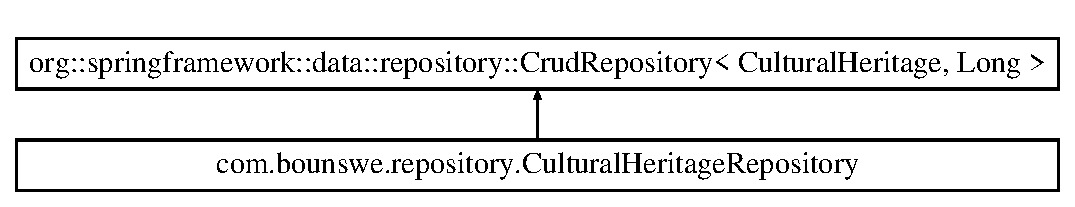
\includegraphics[height=2.000000cm]{interfacecom_1_1bounswe_1_1repository_1_1_cultural_heritage_repository}
\end{center}
\end{figure}


The documentation for this interface was generated from the following file\+:\begin{DoxyCompactItemize}
\item 
src/main/java/com/bounswe/repository/Cultural\+Heritage\+Repository.\+java\end{DoxyCompactItemize}

\hypertarget{classcom_1_1bounswe_1_1controllers_1_1_cultural_heritages_controller}{}\section{com.\+bounswe.\+controllers.\+Cultural\+Heritages\+Controller Class Reference}
\label{classcom_1_1bounswe_1_1controllers_1_1_cultural_heritages_controller}\index{com.\+bounswe.\+controllers.\+Cultural\+Heritages\+Controller@{com.\+bounswe.\+controllers.\+Cultural\+Heritages\+Controller}}
\subsection*{Public Member Functions}
\begin{DoxyCompactItemize}
\item 
\mbox{\Hypertarget{classcom_1_1bounswe_1_1controllers_1_1_cultural_heritages_controller_a6194a7de4bb7a1a331fc8cabfd022d33}\label{classcom_1_1bounswe_1_1controllers_1_1_cultural_heritages_controller_a6194a7de4bb7a1a331fc8cabfd022d33}} 
{\bfseries Cultural\+Heritages\+Controller} (\hyperlink{classcom_1_1bounswe_1_1services_1_1_cultural_heritage_service}{Cultural\+Heritage\+Service} cultural\+Heritage\+Service, \hyperlink{classcom_1_1bounswe_1_1services_1_1_user_service}{User\+Service} user\+Service)
\item 
\mbox{\Hypertarget{classcom_1_1bounswe_1_1controllers_1_1_cultural_heritages_controller_a93a08a5718c76206db576488c1c00829}\label{classcom_1_1bounswe_1_1controllers_1_1_cultural_heritages_controller_a93a08a5718c76206db576488c1c00829}} 
Array\+List$<$ \hyperlink{classcom_1_1bounswe_1_1models_1_1_cultural_heritage}{Cultural\+Heritage} $>$ {\bfseries get\+Cultural\+Heritages} ()
\item 
\mbox{\Hypertarget{classcom_1_1bounswe_1_1controllers_1_1_cultural_heritages_controller_a3179f39e07173126f41d15e143dca0a9}\label{classcom_1_1bounswe_1_1controllers_1_1_cultural_heritages_controller_a3179f39e07173126f41d15e143dca0a9}} 
\hyperlink{classcom_1_1bounswe_1_1models_1_1_cultural_heritage}{Cultural\+Heritage} {\bfseries add\+Cultural\+Heritage} ( @Path\+Variable(value=\char`\"{}user\+Id\char`\"{}) String user\+Id, @Request\+Body \hyperlink{classcom_1_1bounswe_1_1models_1_1_cultural_heritage}{Cultural\+Heritage} cultural\+Heritage)
\item 
\mbox{\Hypertarget{classcom_1_1bounswe_1_1controllers_1_1_cultural_heritages_controller_a6d23f337f8b4cb0292ce81d960083d61}\label{classcom_1_1bounswe_1_1controllers_1_1_cultural_heritages_controller_a6d23f337f8b4cb0292ce81d960083d61}} 
\hyperlink{classcom_1_1bounswe_1_1models_1_1_cultural_heritage}{Cultural\+Heritage} {\bfseries delete\+Item} (@Path\+Variable(value=\char`\"{}item\+Id\char`\"{}) final Long item\+Id)
\item 
\mbox{\Hypertarget{classcom_1_1bounswe_1_1controllers_1_1_cultural_heritages_controller_afb119a1b8434521644c8ab386b98035c}\label{classcom_1_1bounswe_1_1controllers_1_1_cultural_heritages_controller_afb119a1b8434521644c8ab386b98035c}} 
\hyperlink{classcom_1_1bounswe_1_1models_1_1_cultural_heritage}{Cultural\+Heritage} {\bfseries update\+Item} ( @Path\+Variable(value=\char`\"{}item\+Id\char`\"{}) final Long item\+Id, @Request\+Param(value=\char`\"{}title\char`\"{}, default\+Value=\char`\"{}\char`\"{}) String title, @Request\+Param(value=\char`\"{}description\char`\"{}, default\+Value=\char`\"{}\char`\"{}) String description, @Request\+Param(value=\char`\"{}continent\char`\"{}, default\+Value=\char`\"{}\char`\"{}) String continent, @Request\+Param(value=\char`\"{}city\char`\"{}, default\+Value=\char`\"{}\char`\"{}) String city)
\end{DoxyCompactItemize}


The documentation for this class was generated from the following file\+:\begin{DoxyCompactItemize}
\item 
src/main/java/com/bounswe/controllers/Cultural\+Heritages\+Controller.\+java\end{DoxyCompactItemize}

\hypertarget{classcom_1_1bounswe_1_1services_1_1_cultural_heritage_service}{}\section{com.\+bounswe.\+services.\+Cultural\+Heritage\+Service Class Reference}
\label{classcom_1_1bounswe_1_1services_1_1_cultural_heritage_service}\index{com.\+bounswe.\+services.\+Cultural\+Heritage\+Service@{com.\+bounswe.\+services.\+Cultural\+Heritage\+Service}}
\subsection*{Public Member Functions}
\begin{DoxyCompactItemize}
\item 
\mbox{\Hypertarget{classcom_1_1bounswe_1_1services_1_1_cultural_heritage_service_ad77c0b61078a9876dfc71555c56470c6}\label{classcom_1_1bounswe_1_1services_1_1_cultural_heritage_service_ad77c0b61078a9876dfc71555c56470c6}} 
{\bfseries Cultural\+Heritage\+Service} (\hyperlink{interfacecom_1_1bounswe_1_1repository_1_1_cultural_heritage_repository}{Cultural\+Heritage\+Repository} cultural\+Heritage\+Repository)
\item 
\mbox{\Hypertarget{classcom_1_1bounswe_1_1services_1_1_cultural_heritage_service_a0d1ef808dfb1d22c51779231d3d4584a}\label{classcom_1_1bounswe_1_1services_1_1_cultural_heritage_service_a0d1ef808dfb1d22c51779231d3d4584a}} 
Long {\bfseries get\+Count} ()
\item 
\mbox{\Hypertarget{classcom_1_1bounswe_1_1services_1_1_cultural_heritage_service_a4aa90bd1c9843535ccb568666f5b917c}\label{classcom_1_1bounswe_1_1services_1_1_cultural_heritage_service_a4aa90bd1c9843535ccb568666f5b917c}} 
void {\bfseries save} (\hyperlink{classcom_1_1bounswe_1_1models_1_1_cultural_heritage}{Cultural\+Heritage} cultural\+Heritage)
\item 
\mbox{\Hypertarget{classcom_1_1bounswe_1_1services_1_1_cultural_heritage_service_aee2af74cfd889705e38c4efbecfead48}\label{classcom_1_1bounswe_1_1services_1_1_cultural_heritage_service_aee2af74cfd889705e38c4efbecfead48}} 
Array\+List$<$ \hyperlink{classcom_1_1bounswe_1_1models_1_1_cultural_heritage}{Cultural\+Heritage} $>$ {\bfseries find\+All} ()
\item 
\mbox{\Hypertarget{classcom_1_1bounswe_1_1services_1_1_cultural_heritage_service_a221d8db44b3d995ded3362848d8a19ec}\label{classcom_1_1bounswe_1_1services_1_1_cultural_heritage_service_a221d8db44b3d995ded3362848d8a19ec}} 
\hyperlink{classcom_1_1bounswe_1_1models_1_1_cultural_heritage}{Cultural\+Heritage} {\bfseries find\+One} (Long id)
\item 
\mbox{\Hypertarget{classcom_1_1bounswe_1_1services_1_1_cultural_heritage_service_a5697a11cffb74bc7843ec4882711866a}\label{classcom_1_1bounswe_1_1services_1_1_cultural_heritage_service_a5697a11cffb74bc7843ec4882711866a}} 
void {\bfseries delete} (\hyperlink{classcom_1_1bounswe_1_1models_1_1_cultural_heritage}{Cultural\+Heritage} cultural\+Heritage)
\end{DoxyCompactItemize}


The documentation for this class was generated from the following file\+:\begin{DoxyCompactItemize}
\item 
src/main/java/com/bounswe/services/Cultural\+Heritage\+Service.\+java\end{DoxyCompactItemize}

\hypertarget{classcom_1_1bounswe_1_1models_1_1_greeting}{}\section{com.\+bounswe.\+models.\+Greeting Class Reference}
\label{classcom_1_1bounswe_1_1models_1_1_greeting}\index{com.\+bounswe.\+models.\+Greeting@{com.\+bounswe.\+models.\+Greeting}}
\subsection*{Public Member Functions}
\begin{DoxyCompactItemize}
\item 
\mbox{\Hypertarget{classcom_1_1bounswe_1_1models_1_1_greeting_af201c331cafc4511af6d23fe3a69aa96}\label{classcom_1_1bounswe_1_1models_1_1_greeting_af201c331cafc4511af6d23fe3a69aa96}} 
{\bfseries Greeting} (long id, String content)
\item 
\mbox{\Hypertarget{classcom_1_1bounswe_1_1models_1_1_greeting_a0eefa33d43c209e529b3b8db15333198}\label{classcom_1_1bounswe_1_1models_1_1_greeting_a0eefa33d43c209e529b3b8db15333198}} 
long {\bfseries get\+Id} ()
\item 
\mbox{\Hypertarget{classcom_1_1bounswe_1_1models_1_1_greeting_a3f2163dec4d8bfa758853b682a1548b5}\label{classcom_1_1bounswe_1_1models_1_1_greeting_a3f2163dec4d8bfa758853b682a1548b5}} 
String {\bfseries get\+Content} ()
\end{DoxyCompactItemize}


The documentation for this class was generated from the following file\+:\begin{DoxyCompactItemize}
\item 
src/main/java/com/bounswe/models/Greeting.\+java\end{DoxyCompactItemize}

\hypertarget{classcom_1_1bounswe_1_1controllers_1_1_greeting_controller}{}\section{com.\+bounswe.\+controllers.\+Greeting\+Controller Class Reference}
\label{classcom_1_1bounswe_1_1controllers_1_1_greeting_controller}\index{com.\+bounswe.\+controllers.\+Greeting\+Controller@{com.\+bounswe.\+controllers.\+Greeting\+Controller}}
\subsection*{Public Member Functions}
\begin{DoxyCompactItemize}
\item 
\mbox{\Hypertarget{classcom_1_1bounswe_1_1controllers_1_1_greeting_controller_ae24a1e261096fe0f4f9bab2ca0f45206}\label{classcom_1_1bounswe_1_1controllers_1_1_greeting_controller_ae24a1e261096fe0f4f9bab2ca0f45206}} 
\hyperlink{classcom_1_1bounswe_1_1models_1_1_greeting}{Greeting} {\bfseries greeting} (@Request\+Param(value=\char`\"{}name\char`\"{}, default\+Value=\char`\"{}World\char`\"{}) String name)
\end{DoxyCompactItemize}


The documentation for this class was generated from the following file\+:\begin{DoxyCompactItemize}
\item 
src/main/java/com/bounswe/controllers/Greeting\+Controller.\+java\end{DoxyCompactItemize}

\hypertarget{classcom_1_1bounswe_1_1controllers_1_1_greeting_controller_tests}{}\section{com.\+bounswe.\+controllers.\+Greeting\+Controller\+Tests Class Reference}
\label{classcom_1_1bounswe_1_1controllers_1_1_greeting_controller_tests}\index{com.\+bounswe.\+controllers.\+Greeting\+Controller\+Tests@{com.\+bounswe.\+controllers.\+Greeting\+Controller\+Tests}}
\subsection*{Public Member Functions}
\begin{DoxyCompactItemize}
\item 
\mbox{\Hypertarget{classcom_1_1bounswe_1_1controllers_1_1_greeting_controller_tests_a3c06fa081d3ecc8132dc8e061bc2147c}\label{classcom_1_1bounswe_1_1controllers_1_1_greeting_controller_tests_a3c06fa081d3ecc8132dc8e061bc2147c}} 
void {\bfseries greeting\+\_\+when\+Invoked\+With\+Name\+\_\+then\+Says\+Hello\+Name} ()
\end{DoxyCompactItemize}


The documentation for this class was generated from the following file\+:\begin{DoxyCompactItemize}
\item 
src/test/java/com/bounswe/controllers/Greeting\+Controller\+Tests.\+java\end{DoxyCompactItemize}

\hypertarget{class_greeting_tests}{}\section{Greeting\+Tests Class Reference}
\label{class_greeting_tests}\index{Greeting\+Tests@{Greeting\+Tests}}
\subsection*{Public Member Functions}
\begin{DoxyCompactItemize}
\item 
\mbox{\Hypertarget{class_greeting_tests_a31fc148e431a995e4563fbbdb8701b3b}\label{class_greeting_tests_a31fc148e431a995e4563fbbdb8701b3b}} 
void {\bfseries get\+Id\+\_\+when\+Invoked\+By\+Instance\+Creation\+\_\+then\+Get\+ID} ()
\item 
\mbox{\Hypertarget{class_greeting_tests_aa8e3946b3430b046b9b3ea5e92aaab22}\label{class_greeting_tests_aa8e3946b3430b046b9b3ea5e92aaab22}} 
void {\bfseries get\+Content\+\_\+when\+Invoked\+By\+Instance\+Creation\+\_\+then\+Get\+Content} ()
\end{DoxyCompactItemize}


The documentation for this class was generated from the following file\+:\begin{DoxyCompactItemize}
\item 
src/test/java/com/bounswe/models/Greeting\+Tests.\+java\end{DoxyCompactItemize}

\hypertarget{classcom_1_1bounswe_1_1models_1_1_media_item}{}\section{com.\+bounswe.\+models.\+Media\+Item Class Reference}
\label{classcom_1_1bounswe_1_1models_1_1_media_item}\index{com.\+bounswe.\+models.\+Media\+Item@{com.\+bounswe.\+models.\+Media\+Item}}
\subsection*{Public Member Functions}
\begin{DoxyCompactItemize}
\item 
\mbox{\Hypertarget{classcom_1_1bounswe_1_1models_1_1_media_item_a95c1c858582917ff0977ecb0a3eeea41}\label{classcom_1_1bounswe_1_1models_1_1_media_item_a95c1c858582917ff0977ecb0a3eeea41}} 
{\bfseries Media\+Item} (\hyperlink{classcom_1_1bounswe_1_1models_1_1_user}{User} owner, \hyperlink{classcom_1_1bounswe_1_1models_1_1_cultural_heritage}{Cultural\+Heritage} cultural\+Heritage, String url)
\item 
\mbox{\Hypertarget{classcom_1_1bounswe_1_1models_1_1_media_item_aa71764d546a8dffb25eb7c481ffc7abd}\label{classcom_1_1bounswe_1_1models_1_1_media_item_aa71764d546a8dffb25eb7c481ffc7abd}} 
Long {\bfseries get\+Id} ()
\item 
\mbox{\Hypertarget{classcom_1_1bounswe_1_1models_1_1_media_item_ac9644f23a6311ff21085ddcb283a4cbf}\label{classcom_1_1bounswe_1_1models_1_1_media_item_ac9644f23a6311ff21085ddcb283a4cbf}} 
void {\bfseries set\+Url} (String url)
\item 
\mbox{\Hypertarget{classcom_1_1bounswe_1_1models_1_1_media_item_a582f2cbf13f81d4ce9f9b1001f05626a}\label{classcom_1_1bounswe_1_1models_1_1_media_item_a582f2cbf13f81d4ce9f9b1001f05626a}} 
String {\bfseries get\+Url} ()
\item 
\mbox{\Hypertarget{classcom_1_1bounswe_1_1models_1_1_media_item_acae097a89780292100f53c364c7c0d3f}\label{classcom_1_1bounswe_1_1models_1_1_media_item_acae097a89780292100f53c364c7c0d3f}} 
void {\bfseries set\+Cultural\+Heritage} (\hyperlink{classcom_1_1bounswe_1_1models_1_1_cultural_heritage}{Cultural\+Heritage} cultural\+Heritage)
\item 
\mbox{\Hypertarget{classcom_1_1bounswe_1_1models_1_1_media_item_a2d43592e394782cdef7ecd2c22ae3632}\label{classcom_1_1bounswe_1_1models_1_1_media_item_a2d43592e394782cdef7ecd2c22ae3632}} 
\hyperlink{classcom_1_1bounswe_1_1models_1_1_cultural_heritage}{Cultural\+Heritage} {\bfseries get\+Cultural\+Heritage} ()
\item 
\mbox{\Hypertarget{classcom_1_1bounswe_1_1models_1_1_media_item_ac11c651372b6bfa8aea498434a774955}\label{classcom_1_1bounswe_1_1models_1_1_media_item_ac11c651372b6bfa8aea498434a774955}} 
void {\bfseries set\+Owner} (\hyperlink{classcom_1_1bounswe_1_1models_1_1_user}{User} owner)
\item 
\mbox{\Hypertarget{classcom_1_1bounswe_1_1models_1_1_media_item_a0ba8c30c2c1698b2ae8452dee276ec9d}\label{classcom_1_1bounswe_1_1models_1_1_media_item_a0ba8c30c2c1698b2ae8452dee276ec9d}} 
\hyperlink{classcom_1_1bounswe_1_1models_1_1_user}{User} {\bfseries get\+Owner} ()
\end{DoxyCompactItemize}


The documentation for this class was generated from the following file\+:\begin{DoxyCompactItemize}
\item 
src/main/java/com/bounswe/models/Media\+Item.\+java\end{DoxyCompactItemize}

\hypertarget{classcom_1_1bounswe_1_1controllers_1_1_media_item_controller}{}\section{com.\+bounswe.\+controllers.\+Media\+Item\+Controller Class Reference}
\label{classcom_1_1bounswe_1_1controllers_1_1_media_item_controller}\index{com.\+bounswe.\+controllers.\+Media\+Item\+Controller@{com.\+bounswe.\+controllers.\+Media\+Item\+Controller}}
\subsection*{Public Member Functions}
\begin{DoxyCompactItemize}
\item 
\mbox{\Hypertarget{classcom_1_1bounswe_1_1controllers_1_1_media_item_controller_a450b0e313459a507bd78e8f090d2b305}\label{classcom_1_1bounswe_1_1controllers_1_1_media_item_controller_a450b0e313459a507bd78e8f090d2b305}} 
{\bfseries Media\+Item\+Controller} (\hyperlink{classcom_1_1bounswe_1_1services_1_1_media_item_service}{Media\+Item\+Service} media\+Item\+Service, \hyperlink{classcom_1_1bounswe_1_1services_1_1_cultural_heritage_service}{Cultural\+Heritage\+Service} cultural\+Heritage\+Service, \hyperlink{classcom_1_1bounswe_1_1services_1_1_user_service}{User\+Service} user\+Service)
\item 
\mbox{\Hypertarget{classcom_1_1bounswe_1_1controllers_1_1_media_item_controller_a701cffcefc68eb0ce55acea2fe7a3ef2}\label{classcom_1_1bounswe_1_1controllers_1_1_media_item_controller_a701cffcefc68eb0ce55acea2fe7a3ef2}} 
Array\+List$<$ \hyperlink{classcom_1_1bounswe_1_1models_1_1_media_item}{Media\+Item} $>$ {\bfseries get\+Media\+Items} ()
\item 
\mbox{\Hypertarget{classcom_1_1bounswe_1_1controllers_1_1_media_item_controller_a9c0b38769ee6fd53b8f57e8bab5bf944}\label{classcom_1_1bounswe_1_1controllers_1_1_media_item_controller_a9c0b38769ee6fd53b8f57e8bab5bf944}} 
\hyperlink{classcom_1_1bounswe_1_1models_1_1_media_item}{Media\+Item} {\bfseries add\+Media\+Item} ( @Path\+Variable(value=\char`\"{}user\+ID\char`\"{}) String user\+ID, @Path\+Variable(value=\char`\"{}cultural\+Heritage\+ID\char`\"{}) String cultural\+Heritage\+ID, @Request\+Body \hyperlink{classcom_1_1bounswe_1_1models_1_1_media_item}{Media\+Item} media\+Item)
\end{DoxyCompactItemize}


The documentation for this class was generated from the following file\+:\begin{DoxyCompactItemize}
\item 
src/main/java/com/bounswe/controllers/Media\+Item\+Controller.\+java\end{DoxyCompactItemize}

\hypertarget{interfacecom_1_1bounswe_1_1repository_1_1_media_item_repository}{}\section{com.\+bounswe.\+repository.\+Media\+Item\+Repository Interface Reference}
\label{interfacecom_1_1bounswe_1_1repository_1_1_media_item_repository}\index{com.\+bounswe.\+repository.\+Media\+Item\+Repository@{com.\+bounswe.\+repository.\+Media\+Item\+Repository}}
Inheritance diagram for com.\+bounswe.\+repository.\+Media\+Item\+Repository\+:\begin{figure}[H]
\begin{center}
\leavevmode
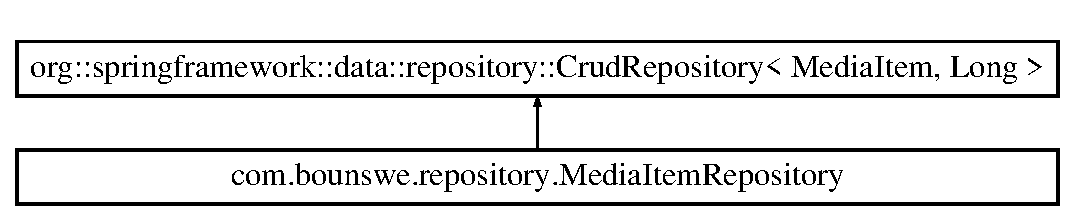
\includegraphics[height=2.000000cm]{interfacecom_1_1bounswe_1_1repository_1_1_media_item_repository}
\end{center}
\end{figure}


The documentation for this interface was generated from the following file\+:\begin{DoxyCompactItemize}
\item 
src/main/java/com/bounswe/repository/Media\+Item\+Repository.\+java\end{DoxyCompactItemize}

\hypertarget{classcom_1_1bounswe_1_1services_1_1_media_item_service}{}\section{com.\+bounswe.\+services.\+Media\+Item\+Service Class Reference}
\label{classcom_1_1bounswe_1_1services_1_1_media_item_service}\index{com.\+bounswe.\+services.\+Media\+Item\+Service@{com.\+bounswe.\+services.\+Media\+Item\+Service}}
\subsection*{Public Member Functions}
\begin{DoxyCompactItemize}
\item 
\mbox{\Hypertarget{classcom_1_1bounswe_1_1services_1_1_media_item_service_ae308dc659369c3f10192481b98f9310e}\label{classcom_1_1bounswe_1_1services_1_1_media_item_service_ae308dc659369c3f10192481b98f9310e}} 
{\bfseries Media\+Item\+Service} (\hyperlink{interfacecom_1_1bounswe_1_1repository_1_1_media_item_repository}{Media\+Item\+Repository} media\+Item\+Repository)
\item 
\mbox{\Hypertarget{classcom_1_1bounswe_1_1services_1_1_media_item_service_a5bd171491671225368bc6479d7a434e3}\label{classcom_1_1bounswe_1_1services_1_1_media_item_service_a5bd171491671225368bc6479d7a434e3}} 
Long {\bfseries get\+Count} ()
\item 
\mbox{\Hypertarget{classcom_1_1bounswe_1_1services_1_1_media_item_service_a0f294e1bca95d36e31add044688106d3}\label{classcom_1_1bounswe_1_1services_1_1_media_item_service_a0f294e1bca95d36e31add044688106d3}} 
void {\bfseries save} (\hyperlink{classcom_1_1bounswe_1_1models_1_1_media_item}{Media\+Item} media\+Item)
\item 
\mbox{\Hypertarget{classcom_1_1bounswe_1_1services_1_1_media_item_service_a906b7a0a40afbc3962cc0e8cf587e2bb}\label{classcom_1_1bounswe_1_1services_1_1_media_item_service_a906b7a0a40afbc3962cc0e8cf587e2bb}} 
Array\+List$<$ \hyperlink{classcom_1_1bounswe_1_1models_1_1_media_item}{Media\+Item} $>$ {\bfseries find\+All} ()
\end{DoxyCompactItemize}


The documentation for this class was generated from the following file\+:\begin{DoxyCompactItemize}
\item 
src/main/java/com/bounswe/services/Media\+Item\+Service.\+java\end{DoxyCompactItemize}

\hypertarget{classcom_1_1bounswe_1_1models_1_1_media_item_tests}{}\section{com.\+bounswe.\+models.\+Media\+Item\+Tests Class Reference}
\label{classcom_1_1bounswe_1_1models_1_1_media_item_tests}\index{com.\+bounswe.\+models.\+Media\+Item\+Tests@{com.\+bounswe.\+models.\+Media\+Item\+Tests}}
\subsection*{Public Member Functions}
\begin{DoxyCompactItemize}
\item 
\mbox{\Hypertarget{classcom_1_1bounswe_1_1models_1_1_media_item_tests_ac837f55ff7f9caa38e53e196b5c73f32}\label{classcom_1_1bounswe_1_1models_1_1_media_item_tests_ac837f55ff7f9caa38e53e196b5c73f32}} 
void {\bfseries get\+Id\+\_\+when\+Instance\+Created\+\_\+then\+Get\+Id} ()
\item 
\mbox{\Hypertarget{classcom_1_1bounswe_1_1models_1_1_media_item_tests_ae6663fed8c78e75f991191e41133f3fb}\label{classcom_1_1bounswe_1_1models_1_1_media_item_tests_ae6663fed8c78e75f991191e41133f3fb}} 
void {\bfseries get\+Url\+\_\+when\+Set\+Url\+Called\+\_\+then\+Get\+Url} ()
\item 
\mbox{\Hypertarget{classcom_1_1bounswe_1_1models_1_1_media_item_tests_a8c86c85ff12cf01a81cbc5f277104b1e}\label{classcom_1_1bounswe_1_1models_1_1_media_item_tests_a8c86c85ff12cf01a81cbc5f277104b1e}} 
void {\bfseries get\+Cultural\+Heritage\+\_\+when\+Set\+Cultural\+Heritage\+Called\+\_\+then\+Get\+Cultural\+Heritage} ()
\item 
\mbox{\Hypertarget{classcom_1_1bounswe_1_1models_1_1_media_item_tests_a3c18e1f83952099ce3e3ae2d7cb6f889}\label{classcom_1_1bounswe_1_1models_1_1_media_item_tests_a3c18e1f83952099ce3e3ae2d7cb6f889}} 
void {\bfseries get\+Owner\+\_\+when\+Set\+Owner\+Called\+\_\+then\+Get\+Owner} ()
\end{DoxyCompactItemize}


The documentation for this class was generated from the following file\+:\begin{DoxyCompactItemize}
\item 
src/test/java/com/bounswe/models/Media\+Item\+Tests.\+java\end{DoxyCompactItemize}

\hypertarget{classcom_1_1bounswe_1_1models_1_1_user}{}\section{com.\+bounswe.\+models.\+User Class Reference}
\label{classcom_1_1bounswe_1_1models_1_1_user}\index{com.\+bounswe.\+models.\+User@{com.\+bounswe.\+models.\+User}}
\subsection*{Public Member Functions}
\begin{DoxyCompactItemize}
\item 
\mbox{\Hypertarget{classcom_1_1bounswe_1_1models_1_1_user_aee7dadb84168d4a5d533bb8eabe98c4d}\label{classcom_1_1bounswe_1_1models_1_1_user_aee7dadb84168d4a5d533bb8eabe98c4d}} 
{\bfseries User} (String first\+Name, String last\+Name)
\item 
\mbox{\Hypertarget{classcom_1_1bounswe_1_1models_1_1_user_a5c9f9c865044921959c2bc3d86fd362d}\label{classcom_1_1bounswe_1_1models_1_1_user_a5c9f9c865044921959c2bc3d86fd362d}} 
{\bfseries User} (String first\+Name, String last\+Name, String email, String user\+Name, String password, String confirm)
\item 
\mbox{\Hypertarget{classcom_1_1bounswe_1_1models_1_1_user_a9a68dfbda052827f9e1666fb1dd5f443}\label{classcom_1_1bounswe_1_1models_1_1_user_a9a68dfbda052827f9e1666fb1dd5f443}} 
void {\bfseries set\+First\+Name} (String first\+Name)
\item 
\mbox{\Hypertarget{classcom_1_1bounswe_1_1models_1_1_user_ad192eeb80ebc0c49a07f4d506fc59234}\label{classcom_1_1bounswe_1_1models_1_1_user_ad192eeb80ebc0c49a07f4d506fc59234}} 
void {\bfseries set\+Last\+Name} (String last\+Name)
\item 
\mbox{\Hypertarget{classcom_1_1bounswe_1_1models_1_1_user_a6e959594820aa26948d4b89250b3c853}\label{classcom_1_1bounswe_1_1models_1_1_user_a6e959594820aa26948d4b89250b3c853}} 
void {\bfseries set\+Email} (String email)
\item 
\mbox{\Hypertarget{classcom_1_1bounswe_1_1models_1_1_user_a4179b291e71b8cd7cde2764fb6ebfbfc}\label{classcom_1_1bounswe_1_1models_1_1_user_a4179b291e71b8cd7cde2764fb6ebfbfc}} 
void {\bfseries set\+User\+Name} (String user\+Name)
\item 
\mbox{\Hypertarget{classcom_1_1bounswe_1_1models_1_1_user_a47430116030529dfb875930050b609eb}\label{classcom_1_1bounswe_1_1models_1_1_user_a47430116030529dfb875930050b609eb}} 
void {\bfseries set\+Password} (String password)
\item 
\mbox{\Hypertarget{classcom_1_1bounswe_1_1models_1_1_user_a54e30a0b48e3296f37f6c1398ca36234}\label{classcom_1_1bounswe_1_1models_1_1_user_a54e30a0b48e3296f37f6c1398ca36234}} 
String {\bfseries get\+Email} ()
\item 
\mbox{\Hypertarget{classcom_1_1bounswe_1_1models_1_1_user_a9c23f1aa306b2813ef33105f61e67c46}\label{classcom_1_1bounswe_1_1models_1_1_user_a9c23f1aa306b2813ef33105f61e67c46}} 
String {\bfseries get\+Name} ()
\item 
\mbox{\Hypertarget{classcom_1_1bounswe_1_1models_1_1_user_a788d42c80d474086bb413feb916afac1}\label{classcom_1_1bounswe_1_1models_1_1_user_a788d42c80d474086bb413feb916afac1}} 
String {\bfseries get\+Password} ()
\end{DoxyCompactItemize}


The documentation for this class was generated from the following file\+:\begin{DoxyCompactItemize}
\item 
src/main/java/com/bounswe/models/User.\+java\end{DoxyCompactItemize}

\hypertarget{interfacecom_1_1bounswe_1_1repository_1_1_user_repository}{}\section{com.\+bounswe.\+repository.\+User\+Repository Interface Reference}
\label{interfacecom_1_1bounswe_1_1repository_1_1_user_repository}\index{com.\+bounswe.\+repository.\+User\+Repository@{com.\+bounswe.\+repository.\+User\+Repository}}
Inheritance diagram for com.\+bounswe.\+repository.\+User\+Repository\+:\begin{figure}[H]
\begin{center}
\leavevmode
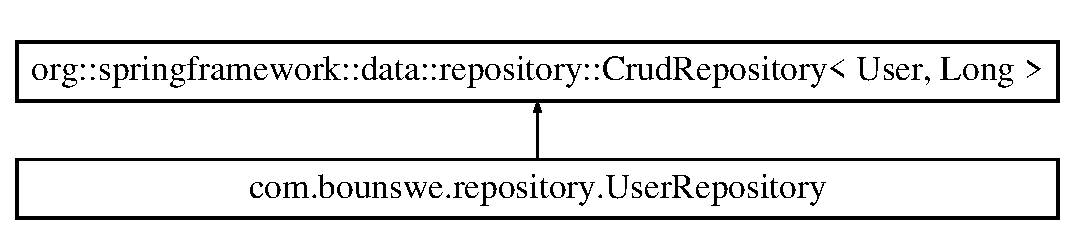
\includegraphics[height=2.000000cm]{interfacecom_1_1bounswe_1_1repository_1_1_user_repository}
\end{center}
\end{figure}


The documentation for this interface was generated from the following file\+:\begin{DoxyCompactItemize}
\item 
src/main/java/com/bounswe/repository/User\+Repository.\+java\end{DoxyCompactItemize}

\hypertarget{classcom_1_1bounswe_1_1controllers_1_1_users_controller}{}\section{com.\+bounswe.\+controllers.\+Users\+Controller Class Reference}
\label{classcom_1_1bounswe_1_1controllers_1_1_users_controller}\index{com.\+bounswe.\+controllers.\+Users\+Controller@{com.\+bounswe.\+controllers.\+Users\+Controller}}
\subsection*{Public Member Functions}
\begin{DoxyCompactItemize}
\item 
\mbox{\Hypertarget{classcom_1_1bounswe_1_1controllers_1_1_users_controller_a0a3434f97661f9d83af2c67521b9b392}\label{classcom_1_1bounswe_1_1controllers_1_1_users_controller_a0a3434f97661f9d83af2c67521b9b392}} 
{\bfseries Users\+Controller} (\hyperlink{classcom_1_1bounswe_1_1services_1_1_user_service}{User\+Service} user\+Service)
\item 
\mbox{\Hypertarget{classcom_1_1bounswe_1_1controllers_1_1_users_controller_ab45fc9120845ffb355d2f1cd901ec364}\label{classcom_1_1bounswe_1_1controllers_1_1_users_controller_ab45fc9120845ffb355d2f1cd901ec364}} 
Array\+List$<$ \hyperlink{classcom_1_1bounswe_1_1models_1_1_user}{User} $>$ {\bfseries get\+Users} ()
\item 
\mbox{\Hypertarget{classcom_1_1bounswe_1_1controllers_1_1_users_controller_a355d0a44de6f7d90145c87f17da675b4}\label{classcom_1_1bounswe_1_1controllers_1_1_users_controller_a355d0a44de6f7d90145c87f17da675b4}} 
Long {\bfseries test} ()
\item 
\mbox{\Hypertarget{classcom_1_1bounswe_1_1controllers_1_1_users_controller_aad6568d2679b1ca7b6608ecb53ed99fe}\label{classcom_1_1bounswe_1_1controllers_1_1_users_controller_aad6568d2679b1ca7b6608ecb53ed99fe}} 
\hyperlink{classcom_1_1bounswe_1_1models_1_1_user}{User} {\bfseries add\+User} (@Request\+Body \hyperlink{classcom_1_1bounswe_1_1models_1_1_user}{User} user)
\end{DoxyCompactItemize}


The documentation for this class was generated from the following file\+:\begin{DoxyCompactItemize}
\item 
src/main/java/com/bounswe/controllers/Users\+Controller.\+java\end{DoxyCompactItemize}

\hypertarget{classcom_1_1bounswe_1_1services_1_1_user_service}{}\section{com.\+bounswe.\+services.\+User\+Service Class Reference}
\label{classcom_1_1bounswe_1_1services_1_1_user_service}\index{com.\+bounswe.\+services.\+User\+Service@{com.\+bounswe.\+services.\+User\+Service}}
\subsection*{Public Member Functions}
\begin{DoxyCompactItemize}
\item 
\mbox{\Hypertarget{classcom_1_1bounswe_1_1services_1_1_user_service_a442d2bb6eec419c795c866ae7c7859c8}\label{classcom_1_1bounswe_1_1services_1_1_user_service_a442d2bb6eec419c795c866ae7c7859c8}} 
{\bfseries User\+Service} (\hyperlink{interfacecom_1_1bounswe_1_1repository_1_1_user_repository}{User\+Repository} user\+Repository)
\item 
\mbox{\Hypertarget{classcom_1_1bounswe_1_1services_1_1_user_service_aeb0c4e4678b50515afa4a5596999cb4f}\label{classcom_1_1bounswe_1_1services_1_1_user_service_aeb0c4e4678b50515afa4a5596999cb4f}} 
Long {\bfseries get\+Count} ()
\item 
\mbox{\Hypertarget{classcom_1_1bounswe_1_1services_1_1_user_service_aa8580f6a3527fccfd1a47f1aa96f9823}\label{classcom_1_1bounswe_1_1services_1_1_user_service_aa8580f6a3527fccfd1a47f1aa96f9823}} 
void {\bfseries save} (\hyperlink{classcom_1_1bounswe_1_1models_1_1_user}{User} user)
\item 
\mbox{\Hypertarget{classcom_1_1bounswe_1_1services_1_1_user_service_ae9c773a0a598946761cd6bab703120d1}\label{classcom_1_1bounswe_1_1services_1_1_user_service_ae9c773a0a598946761cd6bab703120d1}} 
Array\+List$<$ \hyperlink{classcom_1_1bounswe_1_1models_1_1_user}{User} $>$ {\bfseries get\+All\+Users} ()
\item 
\mbox{\Hypertarget{classcom_1_1bounswe_1_1services_1_1_user_service_aefc3b6add70bd0b44113634b1be9fb3d}\label{classcom_1_1bounswe_1_1services_1_1_user_service_aefc3b6add70bd0b44113634b1be9fb3d}} 
\hyperlink{classcom_1_1bounswe_1_1models_1_1_user}{User} {\bfseries find\+One} (Long id)
\end{DoxyCompactItemize}


The documentation for this class was generated from the following file\+:\begin{DoxyCompactItemize}
\item 
src/main/java/com/bounswe/services/User\+Service.\+java\end{DoxyCompactItemize}

\hypertarget{class_user_tests}{}\section{User\+Tests Class Reference}
\label{class_user_tests}\index{User\+Tests@{User\+Tests}}
\subsection*{Public Member Functions}
\begin{DoxyCompactItemize}
\item 
\mbox{\Hypertarget{class_user_tests_a654131cd884303c915b3cd3fda23d6e0}\label{class_user_tests_a654131cd884303c915b3cd3fda23d6e0}} 
void {\bfseries get\+Name\+\_\+when\+Invoked\+By\+Instance\+Creation\+\_\+then\+Get\+Name} ()
\item 
\mbox{\Hypertarget{class_user_tests_ad1b09df79ba0d65d4f217b684f2d45f6}\label{class_user_tests_ad1b09df79ba0d65d4f217b684f2d45f6}} 
void {\bfseries get\+Password\+\_\+when\+Invoked\+By\+Instance\+Creation\+\_\+then\+Get\+Password} ()
\item 
\mbox{\Hypertarget{class_user_tests_af6e52aadfeacf5e299777c653270e824}\label{class_user_tests_af6e52aadfeacf5e299777c653270e824}} 
void {\bfseries get\+Email\+\_\+when\+Invoked\+By\+Instance\+Creation\+\_\+then\+Get\+Email} ()
\end{DoxyCompactItemize}


The documentation for this class was generated from the following file\+:\begin{DoxyCompactItemize}
\item 
src/test/java/com/bounswe/models/User\+Tests.\+java\end{DoxyCompactItemize}

%--- End generated contents ---

% Index
\backmatter
\newpage
\phantomsection
\clearemptydoublepage
\addcontentsline{toc}{chapter}{Index}
\printindex

\end{document}
